\section{Temporal coherence: does the map hold over time?}
\label{sec:temporal}

The map and its strata were both discovered on the baseline visit alone. A map drawn once can
still be a snapshot of nothing: the dimensions might be an artefact of how patients happened to present on the
day they enrolled, the strata a momentary arrangement that dissolves by the next visit. This chapter asks the
question that makes the first two mean something --- does the signal \emph{cohere and persist} over
follow-up? Concretely: does the measurement mean the same thing a year later; which of the nine axes are
\emph{trait-like} (stable, worth stratifying on) versus \emph{state-like} (fluctuating, worth monitoring); and
do the phenotype memberships persist? Throughout, the follow-up visits are scored onto the \emph{fixed} map and
strata --- observed cells only, uncertainty propagated, never re-estimated on later data (invariant
I3). The window is the dense yearly grid V0\,$\to$\,V1\,$\to$\,V2, where all three cohorts are well represented
($9{,}013 \to 4{,}270 \to 2{,}958$ patients). The analysis runs as a sequence of checks --- labelled G1--G6 and
gathered in Table~\ref{tab:m3goals} --- each of which could refute the claim.

\subsection{A geometrically derived, falsifiable prediction}
This is not a fishing expedition. The stratification geometry makes a specific prediction (Figure~\ref{fig:temporalspine}):
if severity is the \emph{spine} the cloud is stretched along, it should be the axis patients move on over time
(state); if the biology axes are fixed phenotype \emph{corners}, they should be the axes patients keep (trait).
Each clause is something the data could refute --- invariance could fail (the map is baseline-specific), the
biology corners could come out noisy (not real phenotypes), the archetypes could dissolve --- which is what
makes this a test rather than a restatement.

\begin{figure}[h]\centering
\temporalspine
\caption{The prediction, made by the stratification geometry. Over follow-up the cohort \emph{slides} along the severity
spine (the population improves --- a state dynamic), while each patient's biological \emph{corner} stays fixed
(a trait). The chapter tests this two independent ways: a variance decomposition (G3) and a per-patient
geometric decomposition (G4).}
\label{fig:temporalspine}
\end{figure}

\subsection{The precondition: the map does not drift (G1)}
A change in a patient's coordinate is interpretable as \emph{patient} change only if the instrument still works
the same way --- otherwise apparent movement is measurement drift. So before interpreting anything, we refit
the simple-structure backbone separately at each visit (z-scored in-sample, since Tucker congruence compares
loading \emph{shape} and is scale-free) and compares the loadings to baseline. This is the temporal analogue of
the map's cross-cohort invariance test, with cohort swapped for visit.

\begin{keyresult}[The map measures the same constructs at follow-up]
Five of the six testable backbone axes are metric-invariant across V0\,$\to$\,V1\,$\to$\,V2 --- severity
($\varphi=0.99$), cognition ($0.99$), metabolic ($0.99$), sleep ($1.00$), developmental ($0.96$). Inflammatory
is \emph{partial} ($\varphi=0.90$): its white-cell differential (white-cell count, monocytes, eosinophils)
drifts --- an acute-phase signature --- so inflammatory change carries a documented caveat. The precondition
holds; the licence to read coordinate change as patient change is earned (Figure~\ref{fig:m3invariance}).
\end{keyresult}

\begin{figure}[h]\centering
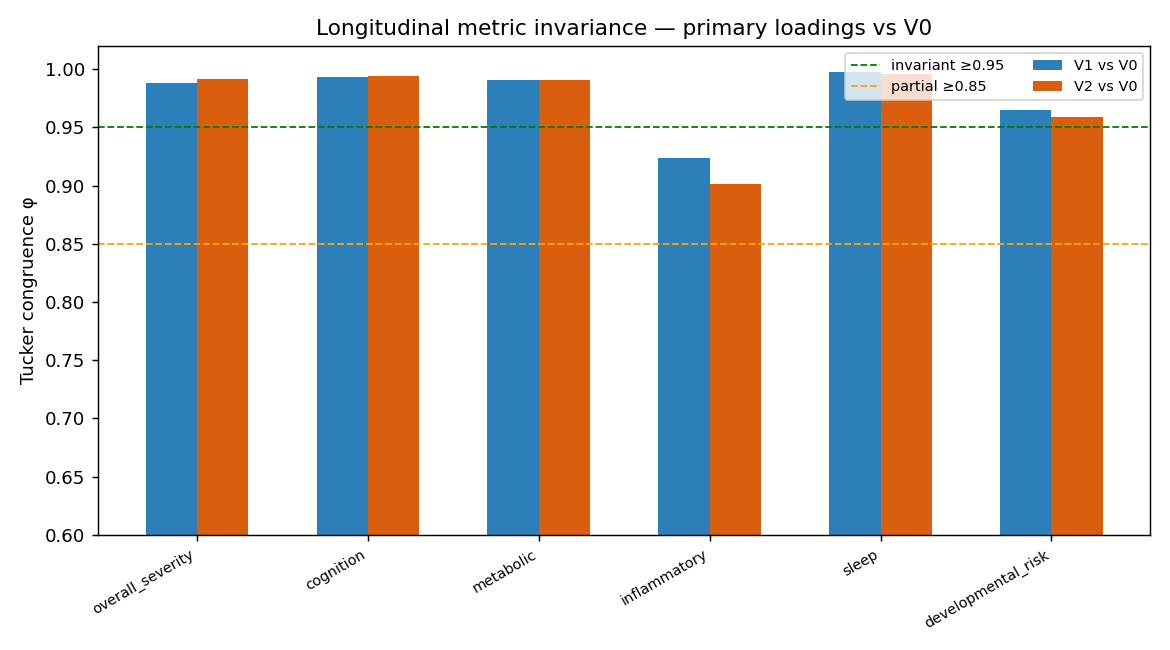
\includegraphics[width=0.86\linewidth]{figures/m3_invariance.png}
\caption{Longitudinal metric invariance. Tucker congruence $\varphi$ of the primary loadings at V1 and V2
against V0, per backbone axis (green band $=$ invariant $\varphi\ge 0.95$, amber $=$ partial). Severity (the
spine) and the trait candidates (cognition, metabolic, developmental) are invariant; only inflammatory drifts.}
\label{fig:m3invariance}
\end{figure}

The three explicit, non-Gaussian axes (suicidality, substance) and thin mania are not backbone-testable; their
change is reported descriptively, never as licensed patient-change.

\subsection{Trait versus state needs two lenses}
\label{sub:traitstate}
For each axis we decompose the longitudinal coordinate into between-patient \emph{trait} variance and
within-patient \emph{state} variance, with the map's measurement error \emph{plugged in} rather than estimated. The
model is a measurement-error random-intercept, with the patient trait integrated out analytically (Gaussian):
\begin{equation}
\label{eq:traitstate}
x_{i,d,t}\;\sim\;\Normal\!\left(\mu_{d,t}+u_{i,d},\;\sigma^2_{w,d}+s^2_{i,d,t}\right),
\qquad u_{i,d}\sim\Normal\!\left(0,\sigma^2_{b,d}\right),
\end{equation}
where $\mu_{d,t}$ are \emph{visit fixed effects} (any population trajectory shape) and $s^2_{i,d,t}$ is the
\emph{known} posterior variance carried over from the map. The trait ratio is the intraclass correlation $\mathrm{ICC}_d =
\sigma^2_{b,d}/(\sigma^2_{b,d}+\sigma^2_{w,d})$.

\begin{methodsbox}[Two design choices that make the answer honest]
Plugging the known $s^2_{i,d,t}$ (rather than letting it inflate $\sigma^2_w$) is what stops a low-reliability
axis from \emph{masquerading} as state --- the correction bites hardest where reliability is low (developmental
raw ICC $0.56\to0.39$ corrected). And the visit fixed effects $\mu_{d,t}$ absorb the \emph{population}
trajectory, so a shared improvement is not miscounted as \emph{individual} instability. That second choice is
what forces the chapter's central nuance.
\end{methodsbox}

The result splits cleanly into two lenses, and the split is the point (Table~\ref{tab:m3traitstate},
Figure~\ref{fig:m3traitstate}):

\begin{itemize}
\item \textbf{Population slide} (the cohort trend $\mu_{d,t}$): the cohort improves on the \emph{symptom/severity}
axes --- suicidality $-0.89$, severity $-0.34$, mania and cognition $\approx-0.16$ --- and is \emph{static on
biology} (metabolic $+0.10$, inflammatory $+0.05$). The cloud slides down severity and symptoms; the biology
stays.
\item \textbf{Individual rank-stability} (ICC, after removing that slide): once the shared improvement is
removed, individual positions are mostly \emph{preserved} --- metabolic $0.93$, inflammatory $0.85$, cognition
$0.78$, severity $0.66$ (trait); sleep $0.49$, suicidality $0.46$, developmental $0.39$ (mixed/state).
\end{itemize}

\begin{table}[h]\centering\small\sffamily
\caption{The trait/state profile, axes ordered state$\to$trait by the individual-rank ICC. ``Slide'' is the
cohort's V0$\to$V2 population trend (removed before the ICC); ``moves'' is the fraction of patients with a
reliable V0$\to$V2 change (Eq.~\ref{eq:rci}); ``licence'' is the G1 verdict. The clean, licensed, predicted-trait
matches --- metabolic and cognition --- land exactly.}
\label{tab:m3traitstate}
\begin{tabular}{L{3.4cm} R{1.3cm} R{1.3cm} R{1.3cm} L{2.0cm} L{2.2cm}}
\toprule
\hdr{axis} & \hdr{ICC} & \hdr{slide} & \hdr{moves} & \hdr{verdict} & \hdr{G1 licence}\\
\midrule
\rowcolor{facebg} developmental & 0.39 & $-0.17$ & 9\% & state\textsuperscript{$\dagger$} & invariant\\
suicidality & 0.46 & $-0.89$ & 32\% & mixed & not tested\\
\rowcolor{facebg} sleep & 0.49 & $-0.08$ & 53\% & mixed & invariant\\
severity (spine) & 0.66 & $-0.34$ & 33\% & trait\textsuperscript{$\ast$} & invariant\\
\rowcolor{facebg} mania & 0.72 & $-0.18$ & 8\% & trait & not tested\\
cognition & \textbf{0.78} & $-0.16$ & 10\% & \textbf{trait} & invariant\\
\rowcolor{facebg} inflammatory & 0.85 & $+0.05$ & 6\% & trait & partial\\
metabolic & \textbf{0.93} & $+0.10$ & 17\% & \textbf{trait} & invariant\\
\rowcolor{facebg} substance & --- & $-0.07$ & 0\% & uninformative & not tested\\
\bottomrule
\end{tabular}
\\[2pt]\footnotesize\raggedright
\textsuperscript{$\ast$}severity is trait by individual rank but slides at the population level (\S\ref{sub:traitstate}).\quad
\textsuperscript{$\dagger$}developmental's ``state'' is a CTQ recall-noise artefact, not change (see caveat below).
\end{table}

\begin{figure}[h]\centering
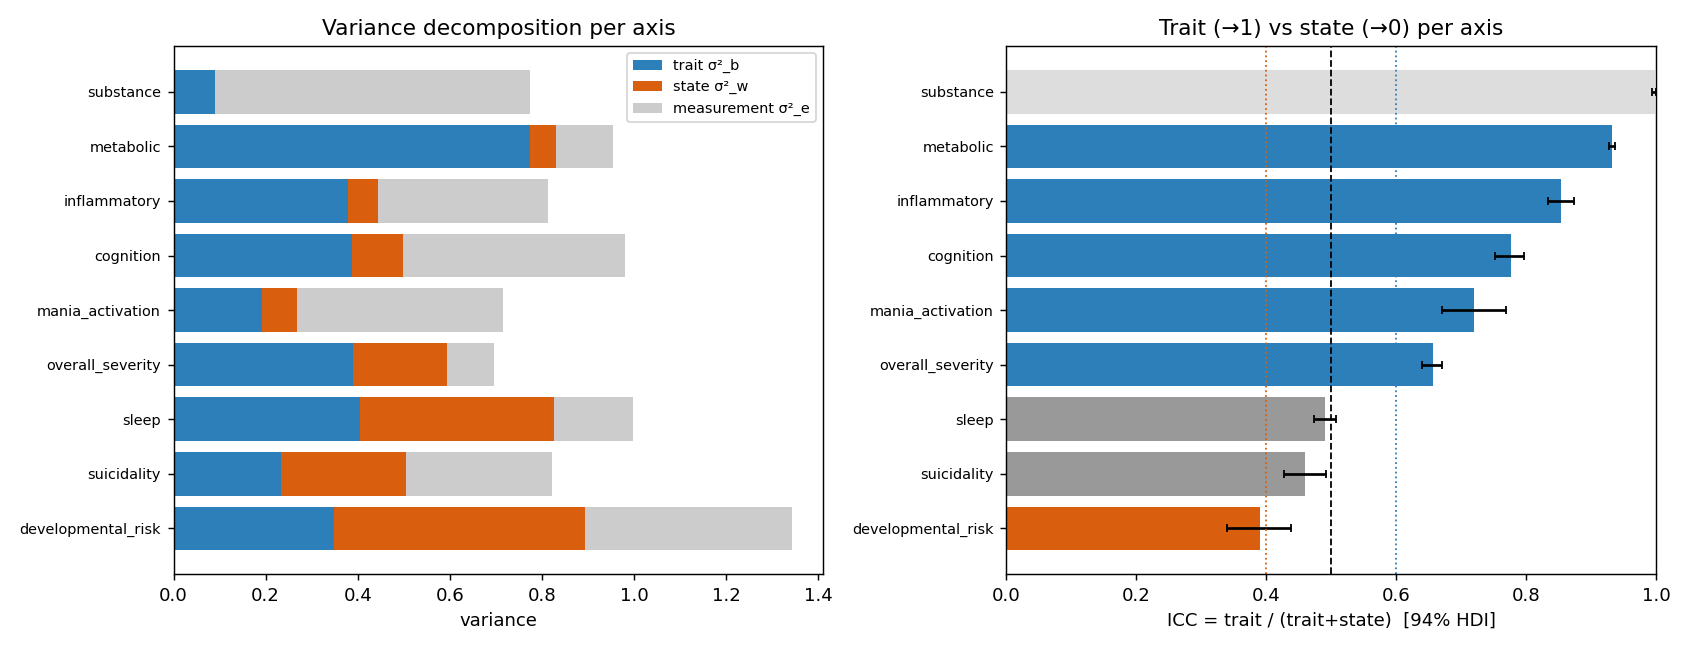
\includegraphics[width=0.96\linewidth]{figures/m3_traitstate.png}
\caption{The variance decomposition. \emph{Left:} between-patient trait, within-person state, and known
measurement variance per axis. \emph{Right:} the trait ratio ICC with 94\% interval (toward $1=$ trait, toward
$0=$ state). Metabolic and cognition are durable; the symptom axes carry more state.}
\label{fig:m3traitstate}
\end{figure}

\begin{caveatbox}[Developmental's ``state'' is measurement, not change]
The model has a blind spot, and the data found it. Childhood trauma is \emph{fixed}, yet developmental came out
the most state-like axis. The plugged variance captures \emph{within-visit} uncertainty, not \emph{cross-visit}
recall inconsistency --- re-administering the childhood-trauma questionnaire produces different answers, and that
wobble lands in $\sigma^2_w$. The tell is that completers (three administrations) look \emph{more} state, not
less; and the reliable-change rule below, robust to sub-band wobble, correctly says developmental holds. The
construct is trait by design; its low ICC is a documented measurement limitation.
\end{caveatbox}

\subsection{The geometry replays: the spine slides, the corners hold (G4)}
\label{sub:spinecorner}
The second, independent route is geometric and per-patient. A coordinate move counts only if it clears
measurement error --- the reliable-change rule
\begin{equation}
\label{eq:rci}
\mathrm{RCI}_{i,d}(s,t)\;=\;\frac{x_{i,d,t}-x_{i,d,s}}{\sqrt{s^2_{i,d,s}+s^2_{i,d,t}}},\qquad
\text{reliable}\iff |\mathrm{RCI}|\ge 1.96 .
\end{equation}
Decomposing each patient's V0$\to$V2 displacement into a movement along the severity spine and a movement in
the biology corner gives the test directly.

\begin{keyresult}[The spine moves, the biology corner holds --- and the archetype persists]
Severity moves reliably in $34.5\%$ of patients; the biology corner (metabolic, inflammatory, cognition) moves
in only $20.2\%$. The predicted cell --- spine moves \emph{while} biology holds --- is $25.8\%$ of patients
versus the anti-pattern (biology moves, spine holds) at $11.5\%$: a $2.2\times$ edge. And the
$G$-residualized (corner-only) archetype identity persists: patients keep their dominant corner phenotype
$52\%$ of the time --- far above the $12.5\%$ chance rate ($\kappa=0.27$, weight-vector cosine $0.81$), as a
soft continuum should (central patients churn their argmax by geometry; the corners stay put)
(Figure~\ref{fig:m3spinecorner}).
\end{keyresult}

\begin{figure}[h]\centering
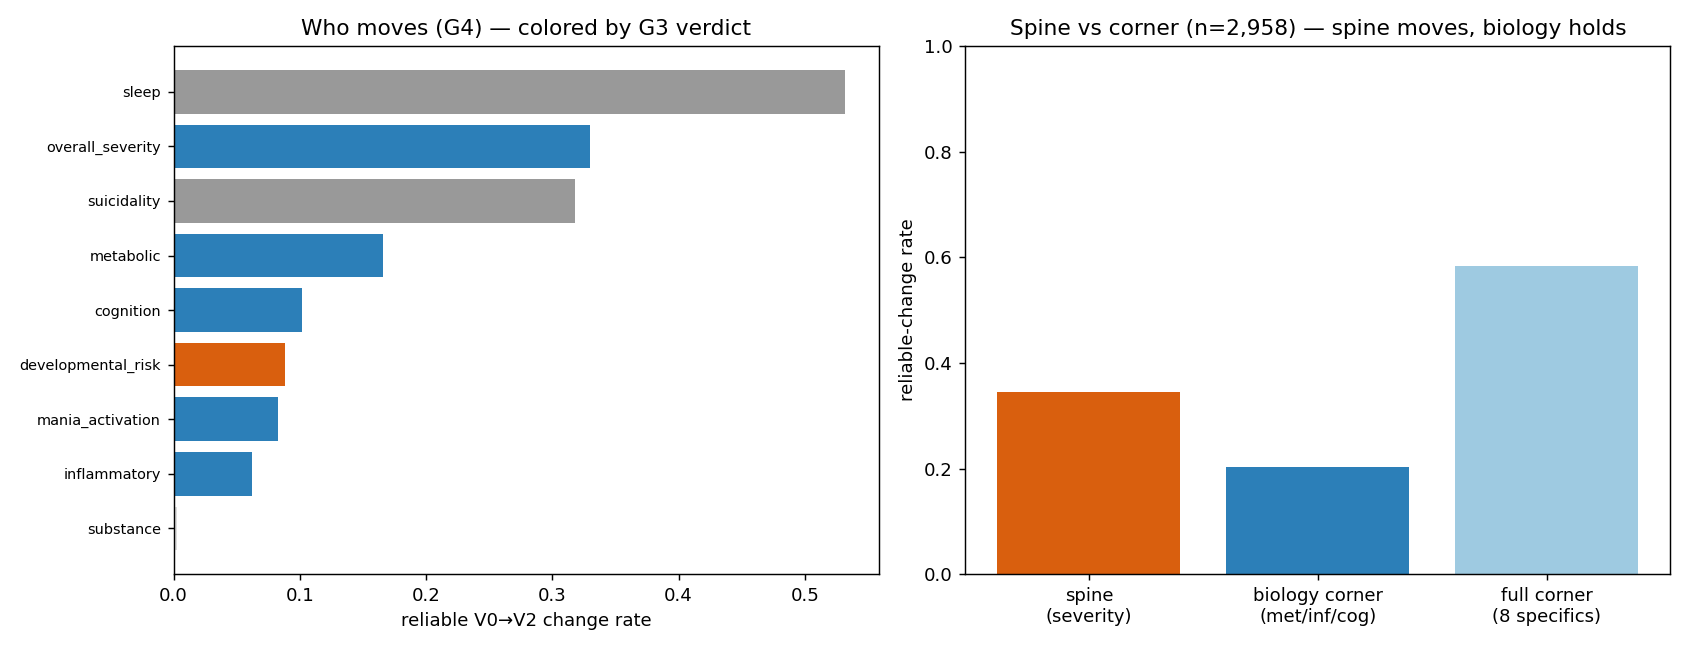
\includegraphics[width=0.96\linewidth]{figures/m3_spinecorner.png}
\caption{Spine-versus-corner. \emph{Left:} the per-axis reliable-change rate, coloured by the G3 trait/state
verdict --- the symptom axes (sleep, severity, suicidality) move, the biology axes hold. \emph{Right:} the
spine moves more than twice as often as the biology corner --- the geometry of ``slide on severity, keep the
phenotype.''}
\label{fig:m3spinecorner}
\end{figure}

\subsection{Two routes, one conclusion}
\label{sub:synthesis}
The real test is whether the variance route (G3) and the geometry route (G4) \emph{agree}. The
simple correlation between an axis's reliable-change rate and its ICC is $\rho=-0.33$ --- the right sign, but
weak --- and the dilution is itself informative, because \emph{exactly two} axes diverge, for reasons we can
name: \textbf{severity} (trait by individual rank, yet it moves via the population slide --- the two routes
measure different things, both correct) and \textbf{developmental} (the recall-noise artefact, where the
reliable-change rule is the more robust route and says it holds). Strip those two principled exceptions and the
core agrees both ways: biology and cognition are durable, the symptom axes move.

\begin{keyresult}[A weak synthesis correlation is the healthier result]
A near-perfect correlation between two operationalizations of the same quantity would signal redundancy, not
corroboration. Two \emph{independent} routes --- a variance decomposition and a geometric one --- agreeing on
the core while diverging for \emph{named} reasons is the stronger evidence. The stratification geometry --- severity the
spine, biology the corners --- is temporally coherent.
\end{keyresult}

\subsection{Honesty: is the retained sample fair? (G6)}
Attrition is the temporal selection threat --- the analogue of the map's completeness concern. If the sicker
systematically dropped out, the retained sample would drift toward health and we could mistake \emph{dropout}
for \emph{improvement}. We regress retention on the nine baseline coordinates.

\begin{keyresult}[Dropout is mild and severity-neutral]
Retention is only weakly predicted by baseline position. Severity is essentially neutral (odds ratio $0.97$ per
SD; the improved do \emph{not} preferentially leave); the one real signal is cognitive impairment (OR $0.83$ ---
the impaired drop out somewhat more); biology is flat. All effects are small ($|d|<0.15$). The trait/state
verdicts are robust completers-versus-all (max $|\Delta\mathrm{ICC}|=0.14$), with inverse-probability weights
available --- so the slide is genuine improvement, not survivorship.
\end{keyresult}

\subsection{What temporal coherence establishes --- and what it defers}
This chapter takes the baseline map and strata and shows they are \emph{temporally coherent}: the measurement holds
across follow-up (G1), and the stratification geometry replays --- the cohort slides on severity and symptoms while
individual biology positions and archetype identity persist --- confirmed two independent ways
(Table~\ref{tab:m3goals}). The operative consequence for what comes next is sharp:
\textbf{stratify on the durable biology (cognition, metabolic, inflammatory); monitor the moving symptoms
(severity, suicidality, sleep).}

\begin{table}[h]\centering\small\sffamily
\caption{The goals and verdicts of this chapter (internal validity, V0$\to$V2). G5 --- a temporal head-to-head against the
diagnostic labels --- is absent by data design: the enrolment diagnosis is time-invariant in the record, so it
is deferred to the prognosis chapter with the diagnosis-change exit signal captured for it.}
\label{tab:m3goals}
\begin{tabular}{L{2.0cm} L{5.4cm} L{5.4cm}}
\toprule
\hdr{goal} & \hdr{question} & \hdr{verdict}\\
\midrule
\rowcolor{facebg} G1 invariance & same constructs at follow-up? & yes --- 5/6 invariant, inflammatory partial\\
G2 substrate & the longitudinal panel & built; V0 reproduces the strata at $99.9\%$\\
\rowcolor{facebg} G3 trait/state & which axes are durable? & biology/cognition trait; severity/symptoms state\\
G4 persistence & spine moves, corner holds? & yes --- $2.2\times$ edge; archetype persists $52\%$\\
\rowcolor{facebg} G3 $\leftrightarrow$ G4 & do the two routes agree? & core yes; two understood exceptions\\
G6 attrition & is the retained sample fair? & dropout mild, severity-neutral\\
\bottomrule
\end{tabular}
\end{table}

\begin{openbox}[Persistence is not prediction --- that comes next]
This chapter establishes that the signal \emph{coheres and persists}; it makes no prognostic, treatment, or external
claim. Whether a baseline coordinate or stratum \emph{predicts} a future outcome --- incrementally beyond
diagnosis and severity --- is the next chapter's question, and the durable axes identified here (cognition, metabolic, inflammatory) are
exactly where that bet is placed. Caveats carried forward: developmental's apparent state is measurement
(recall noise); inflammatory is partial-invariant; substance is uninformative (signal below noise); and the
three-visit window makes trajectory typing coarse. \emph{Persists $\ne$ predicts.}
\end{openbox}
